\documentclass[conference]{IEEEtran}
\IEEEoverridecommandlockouts
% The preceding line is only needed to identify funding in the first footnote. If that is unneeded, please comment it out.
%Template version as of 6/27/2024

\usepackage{cite}
\usepackage{amsmath,amssymb,amsfonts}
\usepackage{algorithmic}
\usepackage{graphicx}
\usepackage{textcomp}
\usepackage{xcolor}
\def\BibTeX{{\rm B\kern-.05em{\sc i\kern-.025em b}\kern-.08em
    T\kern-.1667em\lower.7ex\hbox{E}\kern-.125emX}}
\begin{document}

\title{PRNU: How does Compression degrade Source Camera Identification Performance?
}

\author{\IEEEauthorblockN{Chinasa Njoku}
\IEEEauthorblockA{\textit{Dept. of Artificial Intelligence and Human Interfaces
} \\
\textit{University of Salzburg (PLUS)}\\
J.-Haringerstr.2, 5020 Salzburg, Austria \\
njokuchinasa@gmail.com}
}

\maketitle

\begin{abstract}
With the continued growth and adoption of digital media, the need to attribute digital images to
their sources after they have been acquired remains a fundamental problem in multimedia forensics.
So far, many studies have identified that Source Camera Identification (SCI) using 
Photo Response Non-Uniformity (PRNU) degrades under compression. These studies mostly assess baseline 
JPEG and its impact at different Quality Factors (QFs). However, the challenge is that for a given QF, different images 
compress to different sizes. This is problematic for evaluating the effect of compression in the real-world setting.
In most networks and storage applications the target size is often the fixed parameter while the QF varies per image. 
So in this paper we take a new approach to evaluate the SCI performance under compression at different target bitrates,
simulating real-world strict bandwidth and storage constraints. 
This evaluation is further extended to the more recent compression schemes like JPEG 2000, JPEG XR and JPEG XL.
This proposes a codec recommendation for severe image degradation at very low bitrates that mostly 
preserve the integrity of the forensic signal required for SCI. In addition to the codec recommendation, the robustness
of the PRNU signal is also assessed for both Wavelet and Sigma Filters. For the experiment, the Adobe FiveK dataset 
was used with 17 cameras selected between three different camera brands (NIKON, Canon and Sony). Our results show that JPEGXR had the best forensic performance under mild and severe compression ahead of JPEGXL for the newer codecs. For the older codecs, JPEG had a superior performance over JPEG2000. These performance were largely dependent on the choice of denosing filter and compression algortithm, and less on the resulting quality metrics of the compressed images.   
\end{abstract}

\begin{IEEEkeywords}
Photo Response Non-Uniformity (PRNU), Source Camera Identification (SCI),
image compression, image forensics, image quality metrics.
\end{IEEEkeywords}

\section{Introduction}

Once an image is acquired and shared, it becomes quite difficult to trace back
to the originating sensor if it is not explicitly labeled. Over the years, 
several methods have been developed for reliable SCI.
A very popular technique relies on the unique sensor artifacts that are
present in the image scene. This is also know as the PRNU of the camera.

The PRNU is formed as a result slight microscopic variations in the pixel silicon during manufacturing that causes individual pixels to have different sensitivitiesto light. Therefore once two or more different cameras are used to capture a particular scene,
we can reliably trace which camera generated what image from the noise residue in each image if we know the PRNU reference pattern of the cameras.

This method of SCI is relatively more robust because tracing an image source does not require explicit device
information from the metadata. To identify a source camera, what is needed is only the fixed noise pattern
of the camera.
However, in real world applications the acquired images are rarely in their raw state during source attribution.
In other to store or transfer them over networks, these images undergo compression most times.
Many studies already show that pre-storage or transmission compression after acquisition degrade SCI performance.
But these experiments are mostly based on baseline JPEG and often with fixed QFs. In some cases the effect of the compression are evaluated by compressing already JPEG compressed images. So while this may substantively highlight degrading effect of the forensic signal due to compression, a fixed QF compresses different images to different sizes. This is particularly challenging when evaluating the impact of compression under real-world constraints as most network and storage systems are designed to vary QFs in order to achieve a target bandwidth.

In this work, we propose a more realistic evaluation of the impact of compression on PRNU-based SCI, where the target size is fixed and the QF varies per image. Our assessment also extends to different codecs like JPEG2000, JPEGXR and JPEGXL to evaluate how much of this degradation is codec dependent.

Understanding how different codecs degrade the forensic signal in PRNU is particularly important because they uniquely employ different algorithms and transforms during compression. As show in Fig. 1, the information loss due to compression is different in each codec as a leave different residual error or artifacts on compressed images. For instance the baseline JPEG compression leaves blocky artifacts on the compressed image and is based on 8X8 Discrete Cosine Tranform (DCT) blocks, while JPEG2000 on the other hand is based on the Discrete Wavelet Transform (DWT) and introduces a ringing artifact on the corresponding image.

The more recent codecs like JPEGXR and JPEGXL are also based on Photo Core Transform (PCT) and varying DCT blocks, respectively. Unlike the baseline JPEG with fixed-sized 8X8 pixel blocks, they employ multiple-sized blocks to reduce the blocky artifacts. Specifically, JPEGXL employs an adaptive DCT block from 2X2 to 16X16 blocks depending on image local content and natively includes an inloop edge-preserving filter in the pipeline. JPEGXR also utilizes filters in addition to its hierachichal PCT integer-based blocks. However, these filters are Overlapping and are applied optionally at Pre-Transform and Post-Transform in the pipelines.

These additional processing invariably improve the perceptual quality of the resulting compressed images from both codecs making them increasingly attractive for recent applications over the older JPEG and JPEG2000 codecs. So by evaluating the SCI performance across these codecs, we propose a new benchmark on how each codec preserves the PRNU signal. This is important when making crucial forensic-compliant application and network design decisions.

\begin{figure}[htbp]
\centerline{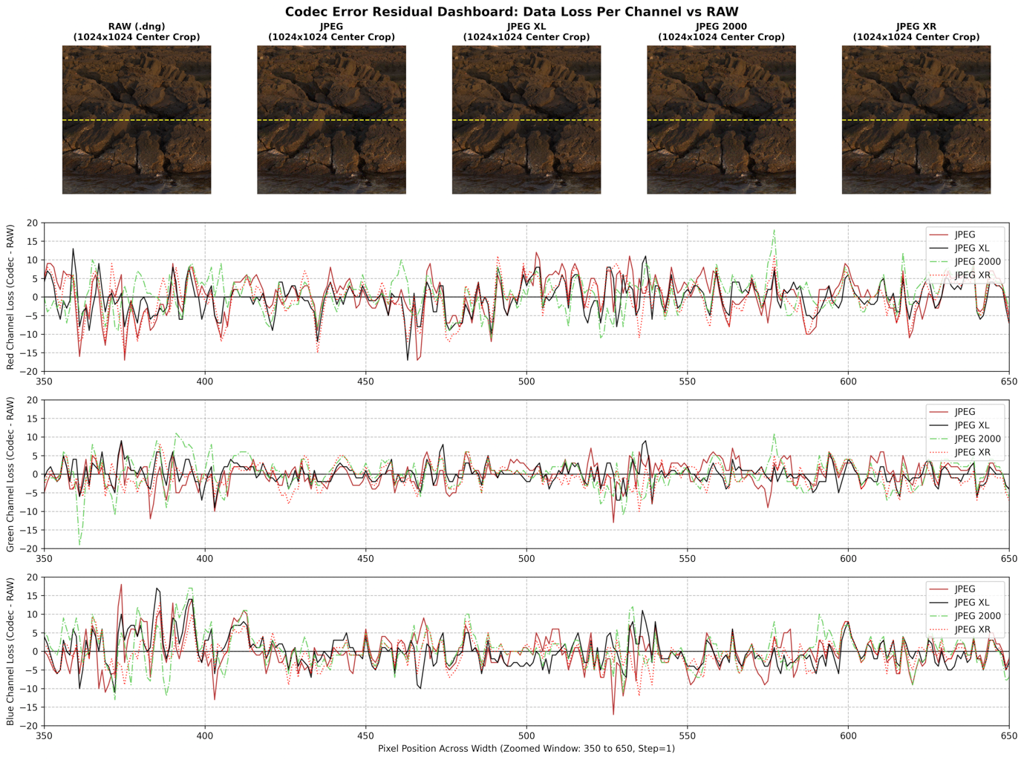
\includegraphics{fig1.png}}
\caption{The residual plot of the center line of a raw image patch of 1024X1024 compressed with JPEG, JPEGXL, JPEG2000 and JPEGXR per color channel.}
\label{fig:prnu_residuals}
\end{figure}

For each codec evaluation, the SCI perforrmance was also computed with both Sigma and Wavelet denoising filters. This shows how much SCI performance depends on the choice denoising filters used in the extraction of residues. In this case, we compare our results from these two filters that have been widely adopted in PRNU research.

The dataset used is from MIT Adobe FiveK database. For statistical relevance, only cameras with images above 70 images each were selected. Such that 50 images are used to build to build the camera reference pattern, while the rest are used to for testing. So in total, 17 cameras and 3,586 images were selected across three different camera brands (NIKON, Canon and Sony).

Once these images were compressed, the quality of each resulting image from each codec was computed for different target sizes. The Signal to Noise Ratio (PSNR) and Structural Similarity Index (SSIM) for non-blind quality metrics and BRISQUE for blind quality scheme.

To match the right camera, the Peak-to-Correlation Energy (PCE) was computed between each image residue and all the reference camera patterns, and the pair with the highest value was declared a match.

The rest of this paper is organised as follows. Section II reviews previous studies on the effect of compression on SCI performance. Then the methodology and experiment setup are described in Section III. Our results and analysis are are presented in Section IV. While in Section V, we make our conclusion our research outcome and propose ideas for future work in this area.

\end{document}


